% docs/texte/20_core/deconvolution.tex -- chapter "Deconvolution" (Interferosim)
% Version: 0.2.0 (2026-10-31) -- package interferosim.deconvolution (interferosim 0.8.0)
%   0.1.0 (2026-10-12): placeholder
% ================================================================
\label{ch:deconvolution-impl}
\index{deconvolution}\index{CLEAN}\index{clean beam}\index{Wiener filter}

H\"ogbom-CLEAN, Wiener filter, clean beam and restoration, comparison
metrics. Implemented in version~0.8.0 in the package
\texttt{interferosim.deconvolution} (classes as in the basic design,
Fig.~\ref{fig:uml-pipeline}); notebook \texttt{07\_deconvolution.ipynb}.
Origin: notebook~A of the teaching material (\texttt{hogbom\_fft}, clean beam
from the main lobe, comparison Wiener against CLEAN). Theory: chapter
\enquote{Deconvolution} in part \enquote{Theory}
(chapter~\ref{ch:deconvolution}).

\section{Implementation}

\begin{description}
  \item[\texttt{Deconvolver}] interface (strategy pattern):
        \texttt{deconvolve(dirty, beam, clean\_beam)} returns a
        \texttt{DeconvResult}; alias \texttt{run} as in the UML diagram.
  \item[\texttt{HogbomClean}] loop gain $g$, iteration limit, stop when the
        residual peak inside the window falls below
        $\max(\text{threshold}, \text{frac}\cdot\text{initial peak})$; CLEAN
        window as boolean mask or circles $(l, m, r)$; option
        \texttt{positive} (only positive peaks). The dirty beam of the
        \texttt{Imager} is periodic in the FFT grid, so the shift to the peak
        is a cyclic roll -- implemented as a slice of the twice-tiled beam
        without copying. The history stores the residual peak and the
        cumulative component flux per iteration.
  \item[\texttt{CleanBeam}] elliptical Gaussian (FWHM of major and minor
        axis, position angle east of north), fitted by least squares to
        $\ln B_D$ of the main-lobe pixels above 0.35; \texttt{kernel},
        \texttt{convolve} (model in Jy/pixel $\to$ image in Jy/beam, a point
        keeps its flux density as peak).
  \item[\texttt{DeconvResult}] model (Jy/pixel), residual and restored image
        $I_R = M * B_C + R$ (Jy/beam), clean beam, number of iterations,
        history; components brightest first, flux within a circle.
  \item[\texttt{WienerFilter}] $\mathcal W = \mathcal S^*/(|\mathcal S|^2 +
        \text{NSR}\cdot\max|\mathcal S|^2)$ with $\mathcal S$ = FFT of the
        dirty beam; \texttt{apply} optionally to the resolution of a target
        clean beam, \texttt{deconvolve} with residual
        $D - \hat I * B_D$.
  \item[\texttt{reference\_image}, \texttt{rms\_error}] the sky model on
        the pixel grid of an image, optionally attenuated per component by
        the primary beam (the apparent sky the visibilities measure) and
        convolved with the clean beam; rms difference within a circle.
\end{description}

\section{Results}

\paragraph*{OH masers with the project baseline.} The maser group of
chapter~\ref{ch:imaging} (natural weighting, grid $512\times0.25''$, loop
gain 0.1, threshold 0.45\,Jy/beam, positive components): CLEAN stops after
297 iterations, the residual has an rms of 0.16\,Jy/beam
(Fig.~\ref{fig:dec-masers}). The reference is the apparent sky: the masers
lie $0.54^\circ$ from the pointing centre, the primary beam of the 3\,m
dishes attenuates them to 0.96 of their flux density.

\begin{center}
\begin{tabular}{@{}lrrrrr@{}}
\toprule
Maser & true [Jy] & apparent & dirty & restored & CLEAN flux \\
\midrule
M1 & 70.0 & 67.0 & 62.0 & 65.4 & 65.3 \\
M2 & 45.0 & 43.0 & 33.7 & 41.0 & 41.2 \\
M3 & 20.0 & 19.1 & 25.3 & 17.9 & 18.0 \\
\midrule
\multicolumn{6}{@{}l}{rms error within $30''$: dirty 8.63, restored 0.19\,Jy/beam} \\
\bottomrule
\end{tabular}
\end{center}
The rms error drops by a factor of about 45. The remaining deficit of
1--2\,Jy per maser is the ambiguity of a single baseline: part of the flux
goes into components at sidelobe positions, where the fringe pattern of
the beam repeats (127 component pixels, 138\,Jy in total).

\begin{figure}[htbp]
  \centering
  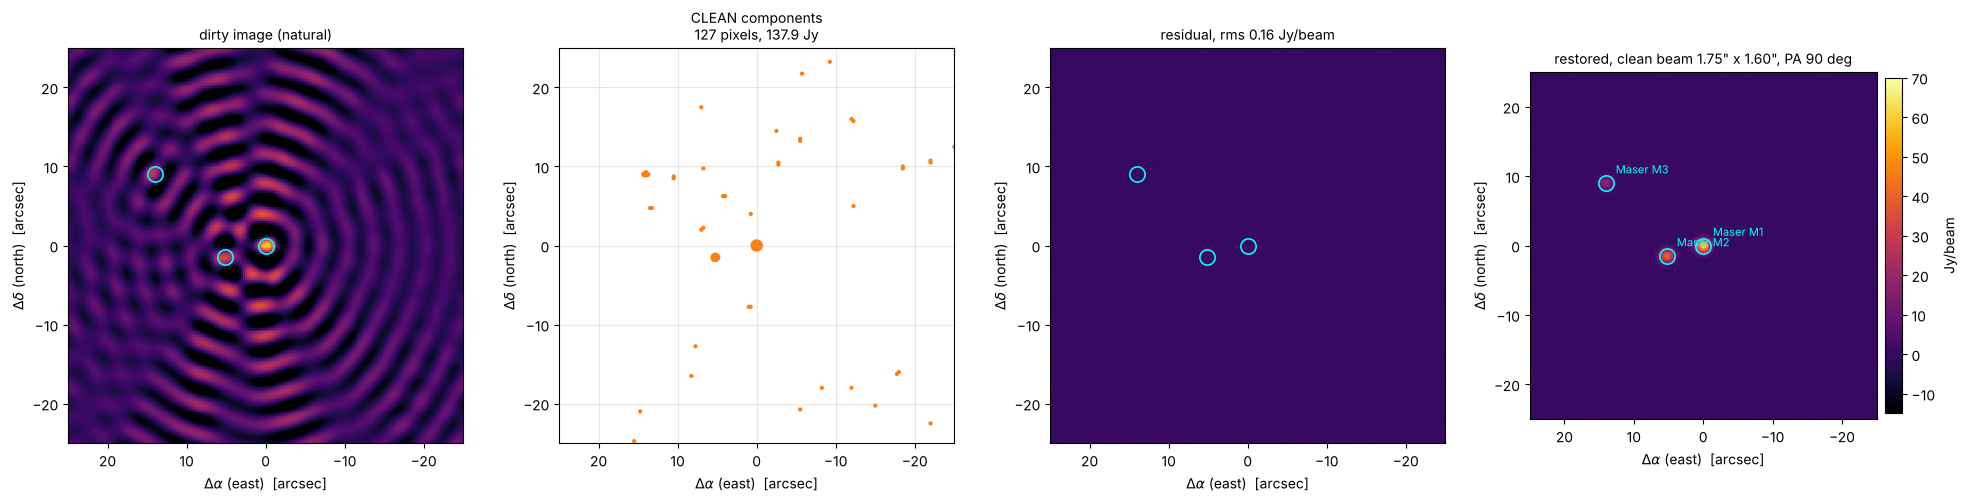
\includegraphics[width=\textwidth]{images/dec_clean_masers.png}
  \caption{CLEAN of the maser group with the project baseline: dirty image,
           CLEAN components (dot area $\propto$ flux), residual, restored
           image; circles: true positions.}
  \label{fig:dec-masers}
\end{figure}

\paragraph*{Convergence and loop gain.} The residual peak falls about
geometrically; $g = 0.05$, 0.1, 0.3 need 594, 297, 103 iterations with the
same rms error (0.19--0.20\,Jy/beam) (Fig.~\ref{fig:dec-gain}).

\begin{figure}[htbp]
  \centering
  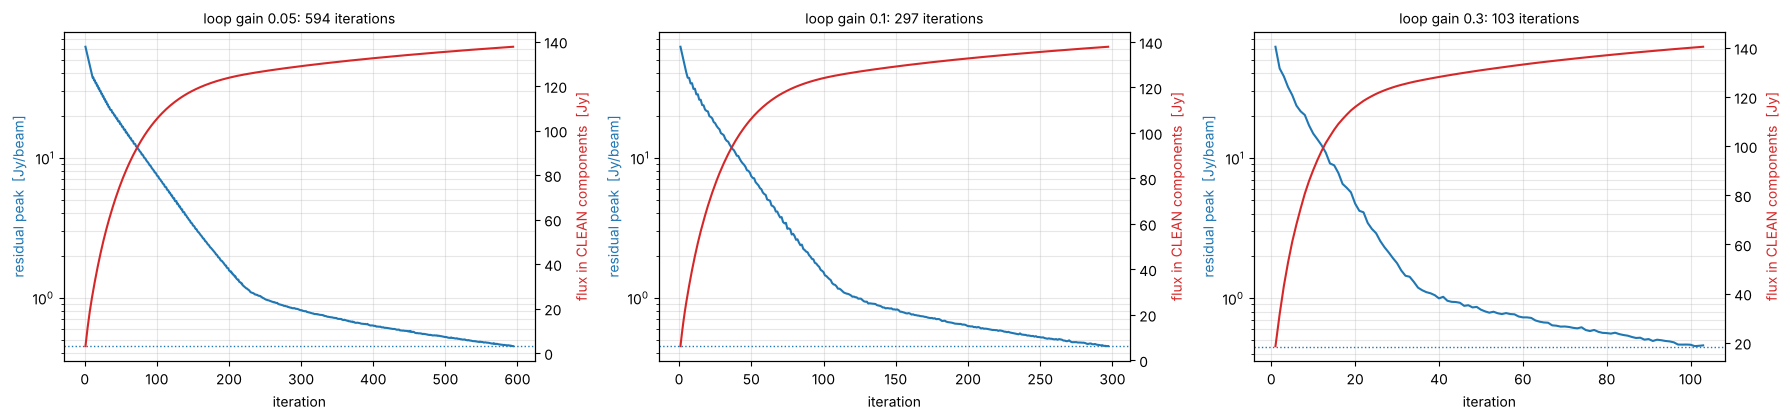
\includegraphics[width=\textwidth]{images/dec_clean_gain.png}
  \caption{Residual peak (blue, threshold dotted) and cumulative CLEAN flux
           (red) against the iteration for three loop gains.}
  \label{fig:dec-gain}
\end{figure}

\paragraph*{Wiener against CLEAN.} As in notebook~A, case~B
(Fig.~\ref{fig:dec-wiener}): only 292 of $512^2$ uv cells (0.11\,\%) are
measured. The Wiener weighting changes the beam only slightly (rms error
8.41\,Jy/beam), the Wiener filter keeps the measured cells and nothing else
-- its image is almost empty (1.3\,Jy/beam at M1). Its small rms error
(1.92\,Jy/beam) is misleading: an empty map is closer to a sparse truth
than a map full of sidelobes. Only the non-linear CLEAN recovers the masers
(0.19\,Jy/beam).

\begin{figure}[htbp]
  \centering
  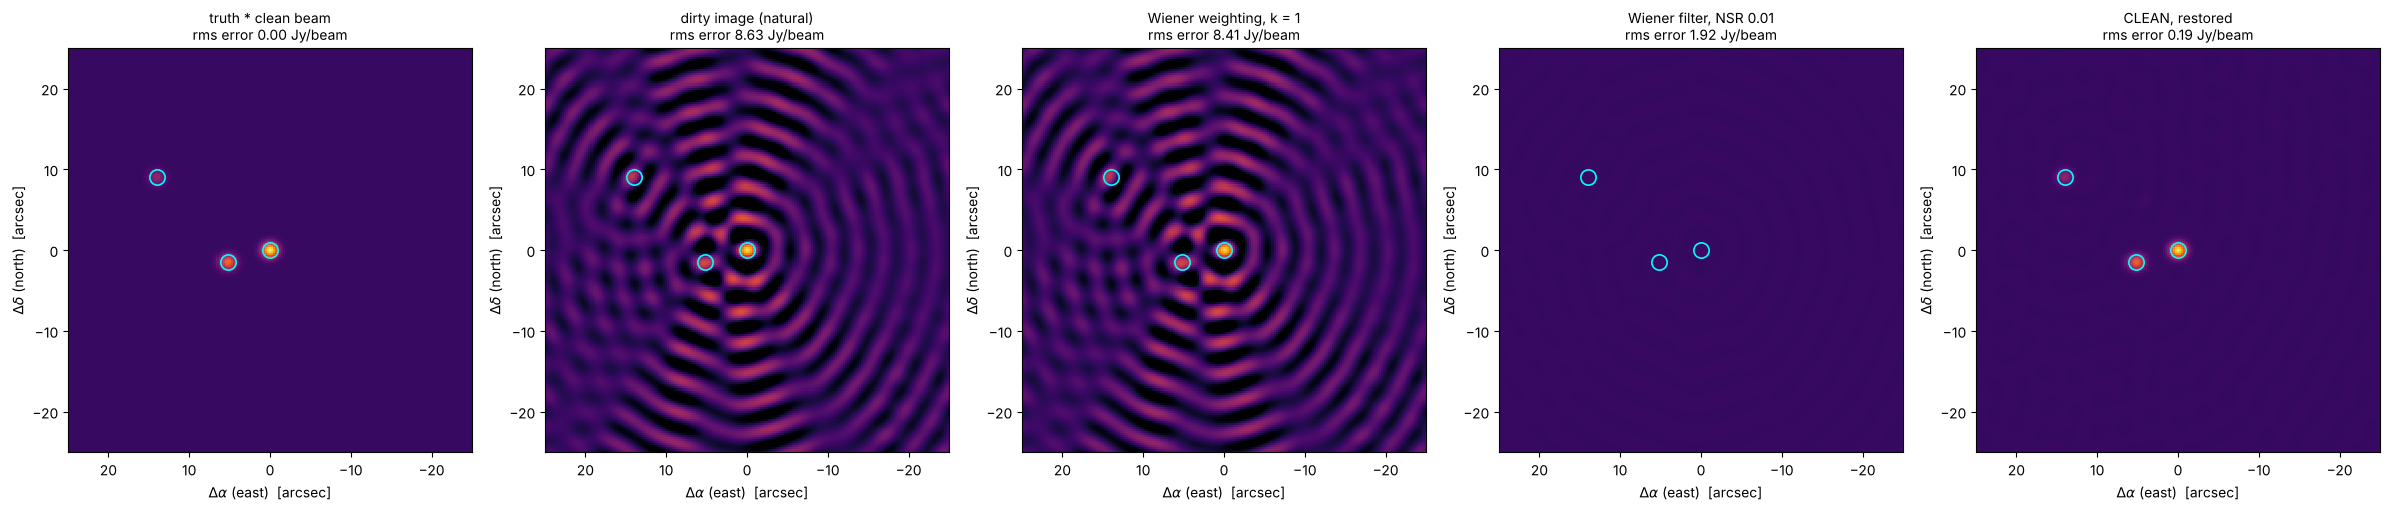
\includegraphics[width=\textwidth]{images/dec_wiener_clean.png}
  \caption{Truth (apparent sky $*$ clean beam), dirty image, Wiener weighting
           ($k=1$), Wiener filter (NSR 0.01, to clean-beam resolution) and
           restored CLEAN image.}
  \label{fig:dec-wiener}
\end{figure}

\paragraph*{More baselines.} With the hypothetical third station the CLEAN
flux densities of the three masers lie within 0.6\,Jy of the apparent ones
(single baseline: within 1.4\,Jy), with fewer spurious components
(Fig.~\ref{fig:dec-three}).

\begin{figure}[htbp]
  \centering
  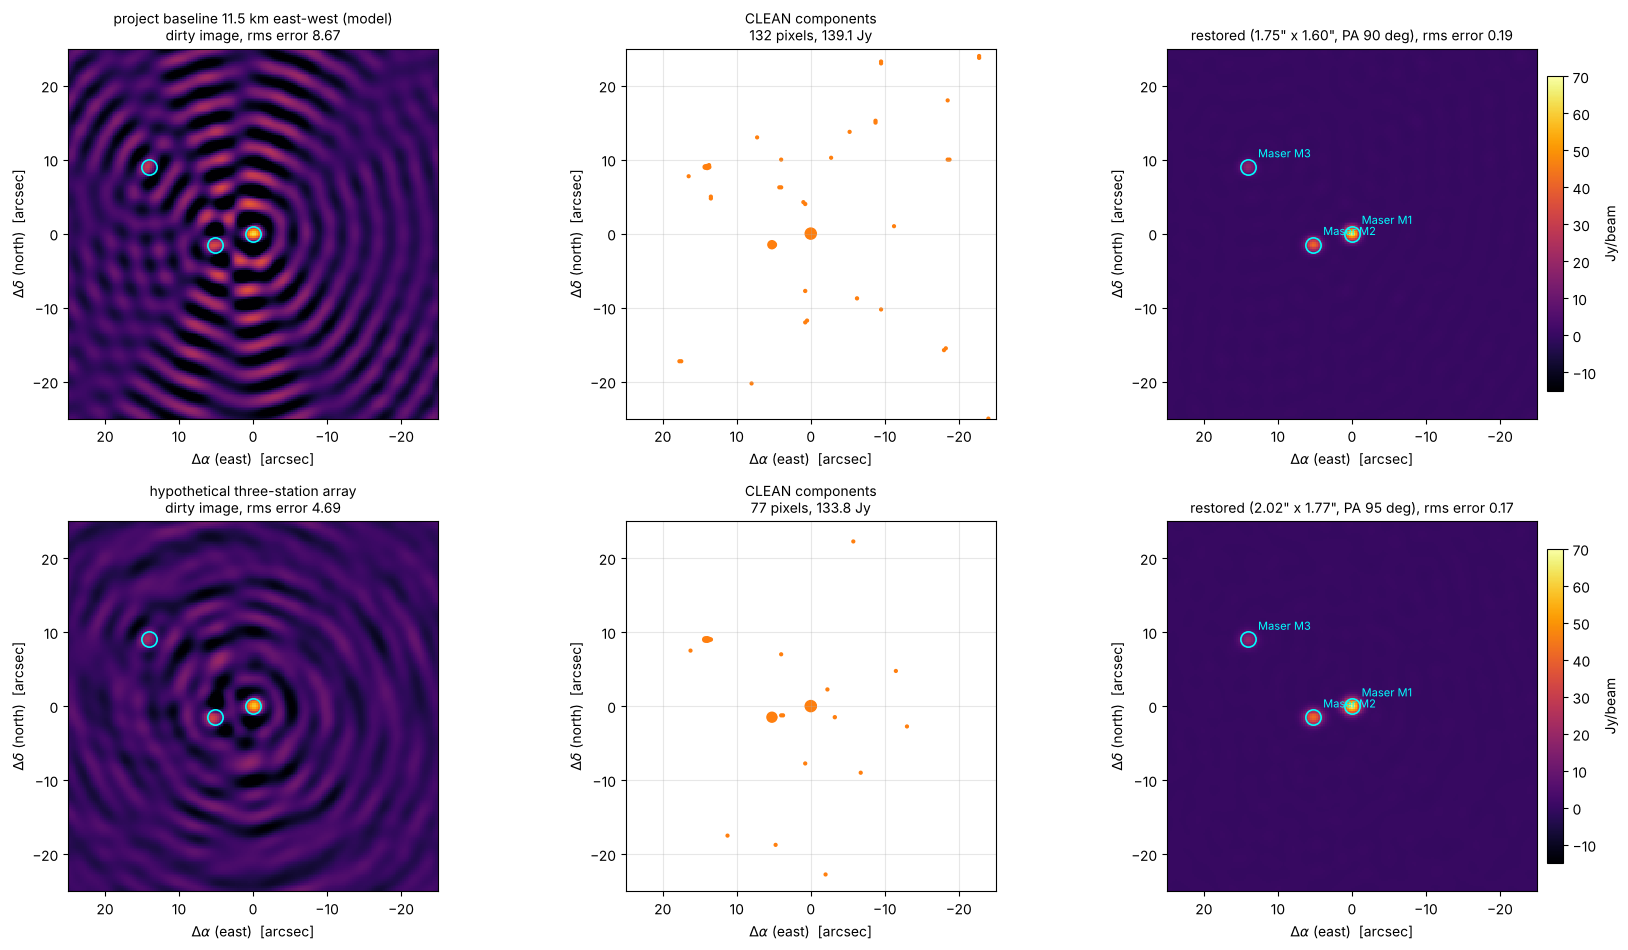
\includegraphics[width=\textwidth]{images/dec_clean_three.png}
  \caption{Project baseline alone (top) and with a hypothetical third station
           (bottom): dirty image, CLEAN components, restored image.}
  \label{fig:dec-three}
\end{figure}

\paragraph*{Limits: Cygnus~A.} CLEAN restores only what its components can
explain from the measured spatial frequencies. At 30--60\,k$\lambda$ the
lobes (${\approx}1400$\,Jy) are resolved out and even the hotspots (FWHM
$3''$) are partly resolved; CLEAN finds 9\,Jy (single baseline) or 49\,Jy
(three stations) of the 1556\,Jy, broken into hundreds of positive and
negative components along the fringes of the beam
(Fig.~\ref{fig:dec-cyga}). The restored image halves the rms error (1.8
$\to$ 0.9\,Jy/beam); with the single baseline its peak is even lower than
the dirty one, because the clean beam averages the alternating components.
Extended emission needs short baselines or single-dish data, and
deconvolution with other priors (multi-scale CLEAN, maximum entropy).

\begin{figure}[htbp]
  \centering
  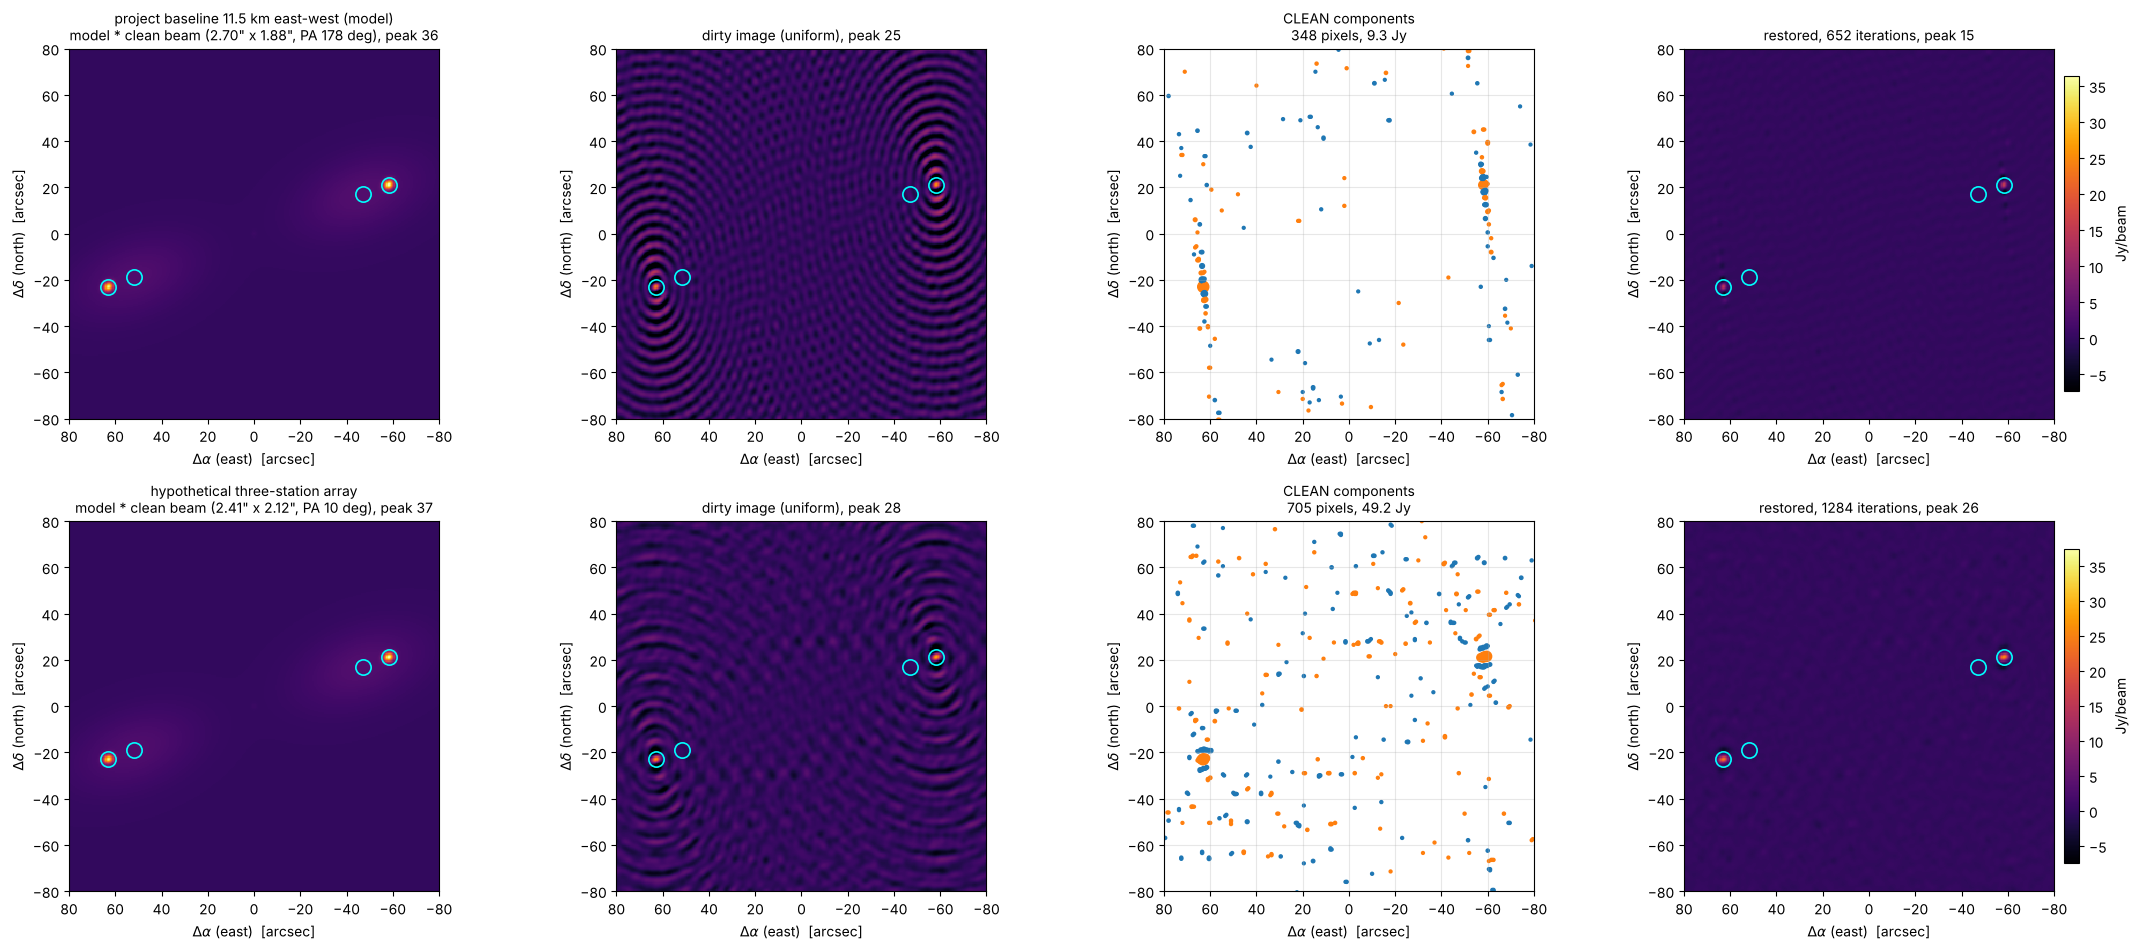
\includegraphics[width=\textwidth]{images/dec_clean_cyga.png}
  \caption{Cygnus~A at 1420\,MHz, project baseline (top) and three stations
           (bottom): apparent model $*$ clean beam, dirty image (uniform),
           CLEAN components (orange positive, blue negative), restored image;
           same colour scale per row.}
  \label{fig:dec-cyga}
\end{figure}
